\documentclass[12pt]{article}
\usepackage[margin=2cm]{geometry}
\usepackage{amsmath}
\usepackage{slashed}
\usepackage{tikz}
\usepackage{verbatim}

\usepackage{hyperref}
\hypersetup{colorlinks=true,urlcolor=blue}

\begin{document}

\noindent
Example 1. Compute the probability $p$ that 23 people have different birthdays.
$$
p=\frac{365}{365}\times\frac{364}{365}\times\frac{363}{365}\times\cdots
\times\frac{343}{365}=\frac{365!/(365-23)!}{365^{23}}
$$

\noindent
The probability that at least two people have the same birthday is $1-p$.

\verbatiminput{example1.txt}

\noindent
To run this script, click on the following link.

\bigskip
\noindent
\url{http://www.eigenmath.org/example1.txt}

\bigskip
\noindent
Then select all text, copy, and paste into the Eigenmath script window.
Then click the Run button.

\begin{center}
\begin{tikzpicture}
\node at (0,0) {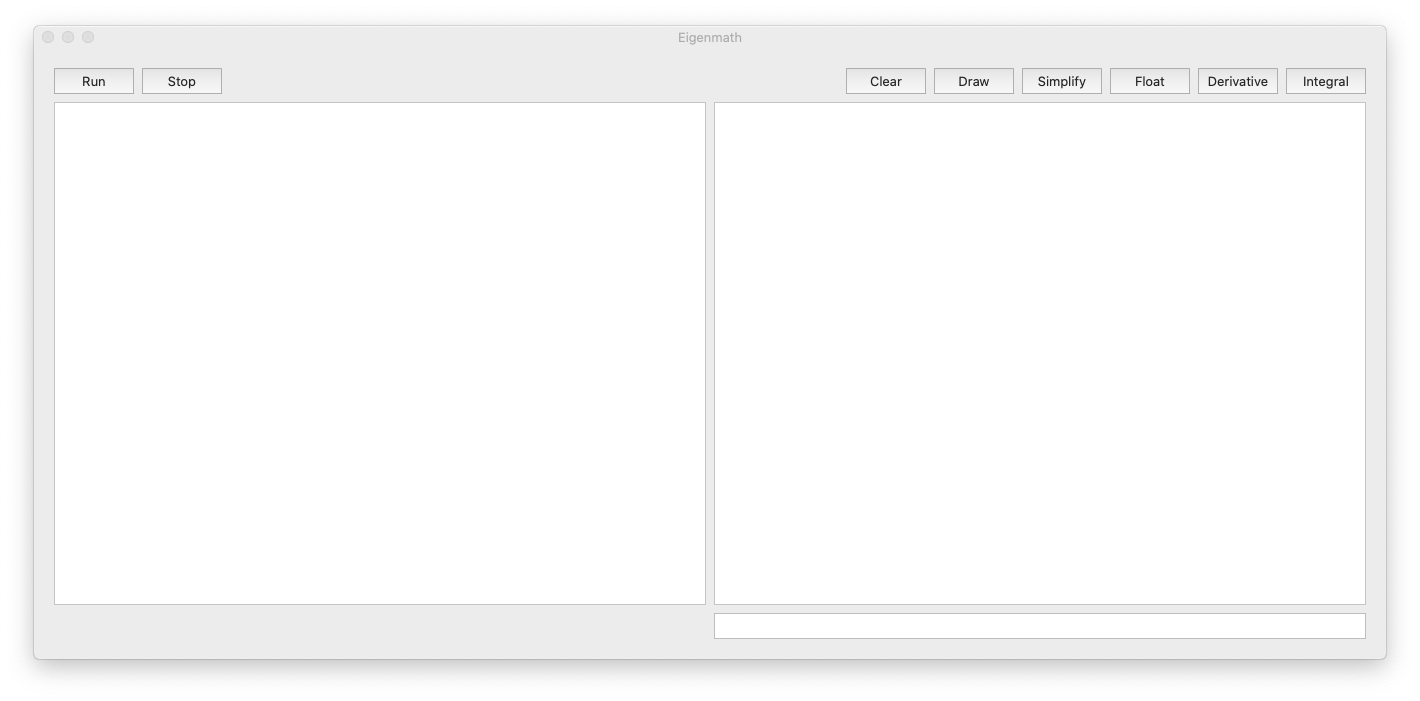
\includegraphics[scale=0.2]{examples-ss1.png}};
\draw (-2.4,0.1) node {Scripts go here.};
%\draw[red,ultra thick,rounded corners] (7.5,5.3) rectangle (9.4,6.2);
\end{tikzpicture}
\end{center}

\newpage
\noindent
Example 2. Show that
$$
\frac{E^2+m^2+p^2\cos\theta}{8p^4}
=\frac{1-\beta^2\sin^2\theta/2}{4p^2\beta^2}
$$
where $p=\sqrt{E^2-m^2}$ and $\beta=p/E$.
The exponential forms of sine and cosine are used
so that trigonometric identities are not needed.

\verbatiminput{example2.txt}

\noindent
\url{http://www.eigenmath.org/example2.txt}

\bigskip
\noindent
Example 3. Let
$$
{\bf E}=
\begin{pmatrix}
A\sin(kz-\omega t+\phi)\\0\\0
\end{pmatrix}
\qquad\text{and}\qquad
{\bf B}=
\begin{pmatrix}
0\\A\sin(kz-\omega t+\phi)\\0
\end{pmatrix}
$$
where $k=\omega/c$.
Verify that $\bf E$ and $\bf B$ are solutions to the free-field Maxwell equations
\begin{gather*}
\nabla\cdot{\bf E}=0\\
\nabla\cdot{\bf B}=0\\
\nabla\times{\bf E}+c^{-1}\frac{\partial}{\partial t}{\bf B}=\begin{pmatrix}0\\0\\0\end{pmatrix}\\
\nabla\times{\bf B}-c^{-1}\frac{\partial}{\partial t}{\bf E}=\begin{pmatrix}0\\0\\0\end{pmatrix}
\end{gather*}

\verbatiminput{example3.txt}

\noindent
\url{http://www.eigenmath.org/example3.txt}

\newpage
\noindent
Example 4. Let
$$
\psi=\exp(ik_xx+ik_yy+ik_zz-i\omega t)
$$

\noindent
where
$$
\omega=\sqrt{k_x^2+k_y^2+k_z^2+m^2}
$$

\noindent
Verify that $\psi$ is a solution to the Klein-Gordon equation
$$
\frac{\partial^2}{\partial t^2}\psi
-\frac{\partial^2}{\partial x^2}\psi
-\frac{\partial^2}{\partial y^2}\psi
-\frac{\partial^2}{\partial z^2}\psi
+m^2\psi=0
$$

\verbatiminput{example4.txt}

\noindent
\url{http://www.eigenmath.org/example4.txt}

\newpage
\noindent
Example 6. Show that
$$
u_1\bar{u}_1+u_2\bar{u}_2=(E+m)(\slashed{p}+m)
$$

\noindent
where
$$
E=\sqrt{p_x^2+p_y^2+p_z^2+m^2}
$$

\noindent
The spinors are
$$
u_1=\begin{pmatrix}E+m\\0\\p_z\\p_x+ip_y\end{pmatrix}
\qquad
u_2=\begin{pmatrix}0\\E+m\\p_x-ip_y\\-p_z\end{pmatrix}
$$

\noindent
The adjoint of $u$ is $\bar{u}=u^\dag\gamma^0$.
Note that $\bar{u}$ is a row vector hence $u\bar{u}$ is an outer product.
This problem demonstrates a trick regarding normalization constants.
The normalization constant $E+m$ is placed on the right-hand side of the equation
instead of normalizing the spinors with $1/\sqrt{E+m}$.
This is because the software is better at simplifying expressions with multipliers
instead of divisors.

\verbatiminput{example6.txt}

\noindent
\url{http://www.eigenmath.org/example6.txt}

\end{document}
